\begin{frame}[containsverbatim]
\begin{center}
\textbf{How to write a project proposal ?}
\end{center}
\end{frame}

\subsection{How to write a project proposal}

\begin{frame}[containsverbatim]
	\frametitle{Structure of a (good) project proposal}	

\begin{itemize}
	\item{(Administration) Who submits it ?}
	\item{(Scientific : Background) From where do we come ?}
	\item{(Scientific : Outcome) Where do we go ?}
	\item{(Technical : Application) What do we  have, how it is implemented ?}
	\item{(Technical : Performance) Why do we need a high-end machine ?}
	\item{(Technical : Resource budget) How much do we need ?}
\end{itemize}

\end{frame}



\subsection{Administrative stuff}

\begin{frame}[containsverbatim]
	\frametitle{Project title}

\begin{itemize}
	\item {Keep it as explicit as possible}
	\item {Propose an accronym (8 letters) : often used as group name}
	\item {Follow the Computing Center's rules}
	\item{\textcolor{dkgreen}{\textit{A High Performance Implementation of a 2D Elliptic Equation Solver: the Poisson's Equation Case at Scale}. Acronym : POISSON} }
	\item{\textcolor{dkred}{\textit{Implementation of a Generic Poisson Solver}. Acronym : POISSON} }
\end{itemize}


\end{frame}



\begin{frame}[containsverbatim]
	\frametitle{Intro cartouche}

The goal is to have the basic administrative stuff and the main requests at a first glance

\begin{center}
\begin{tabular}{| l | l |}
	\hline
	Principal investigator & Vincent Keller, PhD \\
	\hline
	Institution & \'Ecole Polytechnique F\'ed\'erale de Lausanne \\
	\hline
	Laboratory & Scientific IT and Application Support \\
	\hline
	Adress & Station 1, CH-1015 LAUSANNE \\
	\hline
	Involved researchers & Nicolas Richart, PhD ; Christian Cl\'emen\c{c}on \\
	\hline
	Date of submission & April 13, 2015 \\
	\hline
	Expected end of project & October 13, 2015 \\
	\hline
	Target machine & CADMOS Blue Gene Q \\
	\hline
	Proposed acronym & ACRO \\
	\hline
\end{tabular}
\end{center}
\end{frame}


\subsubsection{PI, involved people, institution, CV's}


\begin{frame}[containsverbatim]
	\frametitle{Intro cartouche : Good / Bad practices}

\begin{itemize}
	\item{\textcolor{dkgreen}{Keep it as short as possible}}
	\item{\textcolor{dkgreen}{PI + Key personnel, institution(s), start/end of project, summary of the technical request}}
	\item{\textcolor{dkred}{Not too many details}}
	\item{\textcolor{dkred}{CVs of the project members (put them in an approriate appendix)}}
	\item{\textcolor{dkred}{Potential Collaborations}}
\end{itemize}
\end{frame}



\subsection{Scientific background}

\begin{frame}[containsverbatim]
	\frametitle{Scientific background}
\begin{itemize}
	\item{\textbf{Most important section of the proposal}}
	\item{You and your fellow research scientists or engineers are aware if your research deserves to get computing power}
	\item{To help you : 
	\begin{itemize}
		\item{Good abstract}
		\item{Description of the project}
		\item{References}
	\end{itemize}
	}
%	\item{}
\end{itemize}
\end{frame}


\subsubsection{Abstract}

\begin{frame}[containsverbatim]
	\frametitle{Abstract}

\begin{itemize}
	\item{\textcolor{dkgreen}{ Explicitly express the link between the scientific background and the technical request}}
	\item{\textcolor{dkgreen}{ 500 words max. } }
	\item{\textcolor{dkgreen}{ Assume the reader has little/no knowledge about the technical part and/or the scientific matter} }
	
	\item{\textcolor{dkred}{No copy/paste from previous publications}}
%	\item{\textcolor{red}{}}
%	\item{\textcolor{red}{}}
%	\item{\textcolor{red}{}}
\end{itemize}
\end{frame}


\subsubsection{Description of the project}

\begin{frame}[containsverbatim]
	\frametitle{Description of the project}

\begin{itemize}
	\item{\textcolor{dkgreen}{Description of the research/production project} }
	\item{\textcolor{dkgreen}{Motivation}
		\begin{itemize}
			\item{My project uses an existing, known and well-tested code (Production project)}
			\item{My project will explore a new paradigm at scale (exploratory project)}
			\item{My project has never been tested at scale, needs improvements from an existing code (research project)}
		\end{itemize}
	}
	\item{\textcolor{dkgreen}{Computational objectives} }
	\item{\textcolor{dkgreen}{Expected innovations both at scientific and computational levels} }
%	\item{\textcolor{red}{}}
%	\item{\textcolor{red}{}}
%	\item{\textcolor{red}{}}
\end{itemize}
\end{frame}


\begin{frame}[containsverbatim]
	\frametitle{Scientific background and outcome}
\textbf{Most important point : this part is usually peer-reviewed by a pool of experts/reviewers from the domain.}
\begin{itemize}
	\item{\textcolor{dkgreen}{State-of-the-art review} }
	\item{\textcolor{dkgreen}{Extensive references} }
	\item{\textcolor{dkgreen}{Current status on the subject}	} 
	\item{\textcolor{dkred}{``We are the only ones in the world doing that and you are too stupid to understand it''} }
%	\item{\textcolor{red}{}}
%	\item{\textcolor{red}{}}
%	\item{\textcolor{red}{}}
\end{itemize}
\end{frame}



\subsection{Technical part}

\begin{frame}[containsverbatim]
	\frametitle{Technical part}

Technical part of the project proposal. What is the \textbf{application} you are planning to run on the target architecture ?

\begin{itemize}
	\item{What code (application) are we planning to use }
	\item{Numerical methods
		\begin{itemize}
			\item{ FEM, SEM, FDM, LBM, SPH, MD, etc..}
		\end{itemize}
	}
	\item{Algorithms
		\begin{itemize}
			\item{ Describe the main algorithms}
			\item{ Main bottlenecks and how they have been tackled}
		\end{itemize}
	}
	\item{Implementation 
		\begin{itemize}
			\item{ Pure MPI, GPU, OpenMP, hybrid ? ...}
			\item{ Does it use special libraries ? }
		\end{itemize}
	}
	\item{If third-party code : name, version and license. Your contact within the third-party company/institution}
\end{itemize}
\end{frame}





\subsection{Performance}


\begin{frame}[containsverbatim]
	\frametitle{Performance expectations}

This section should explain how your code behaves and the accuracy with what you request.

\begin{itemize}
	\item { theoretical complexity: communication and computation complexities }
	\item { weak scaling : behavior of the application by fixing the size of the problem per processor and increasing the number of processors: \textbf{parallel efficiency} ($E_p = S_p/p$) }
	\item { strong scaling : behavior of the application by fixing the total size of the problem and increasing the number of processors: \textbf{speedup} ($S_p = t_1/t_p$) }
\end{itemize}
\end{frame}


\subsubsection{Theoretical complexity}


\begin{frame}[containsverbatim]
	\frametitle{Benchmarking}


\begin{itemize}
	\item { You get access to a \textbf{test partition} which allows you to run test cases and measure the performance }
	\item { You also have previous performance measurements from the development }
	\item { Benchmarking is done on larger enough problems, closer to what will be done in production }
	\item { Use the theoretical complexities (computation and communication) to predict how your application will behave at production scale }
\end{itemize}
\end{frame}



\subsubsection{Strong scaling}


\begin{frame}[containsverbatim]
	\frametitle{Strong scaling : Good example (with speedup)}

\begin{columns}
\column{0.5\textwidth} %first column
\begin{center}
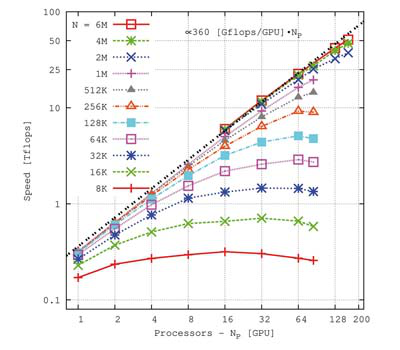
\includegraphics[width=5cm]{Day4/images/strong-good2.png}
\end{center}

\column{0.5\textwidth} %second column
\begin{itemize}
	\item {log-log graph}
	\item {Different problem sizes}
	\item {linear regression curves}
\end{itemize}
\end{columns}
\textbf{Source: HLRS \url{http://inside.hlrs.de/_old/htm/Edition_01_12/article_20.html}}

\end{frame}


\begin{frame}[containsverbatim]
	\frametitle{Strong scaling : Good example (with timing)}

\begin{columns}
\column{0.5\textwidth} %first column
\begin{center}
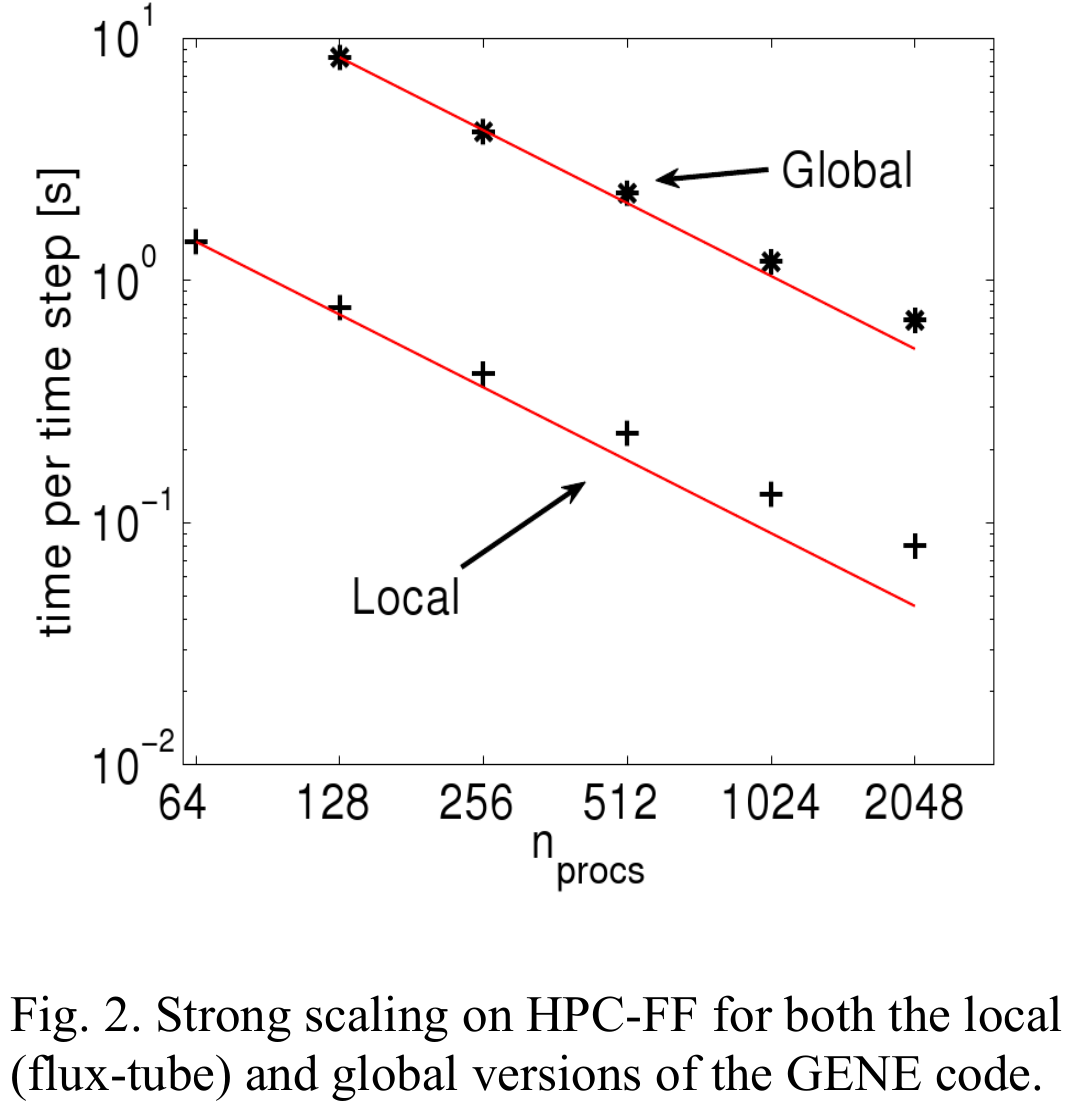
\includegraphics[width=6cm]{Day4/images/strong-good.png}
\end{center}

\column{0.5\textwidth} %second column
\begin{itemize}
	\item {log-log graph}
	\item {time \textbf{per step}}
	\item {explicit caption}
	\item {linear regression curves}
\end{itemize}
\end{columns}
\textbf{Source: CRPP, EPFL, Project proposal for BG/P, 2011}

\end{frame}


\begin{frame}[containsverbatim]
	\frametitle{Strong scaling : bad example}

\begin{columns}
\column{0.5\textwidth} %first column
\begin{center}
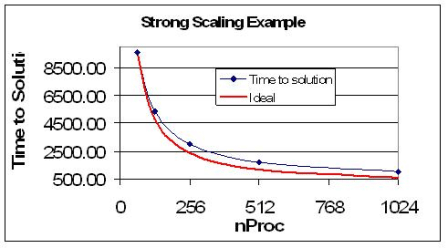
\includegraphics[width=5cm]{Day4/images/strong-bad.png}
\end{center}

\column{0.5\textwidth} %second column
\begin{itemize}
	\item {linear scale}
	\item {no caption}
	\item {``Excel'' look}
	\item {useless for any conclusion}
\end{itemize}
\end{columns}

\end{frame}


\subsubsection{Weak scaling}

\begin{frame}[containsverbatim]
	\frametitle{Weak scaling : Good example (FZJ J\"ulich, Germany)}

\begin{columns}
\column{0.5\textwidth} %first column
\begin{center}
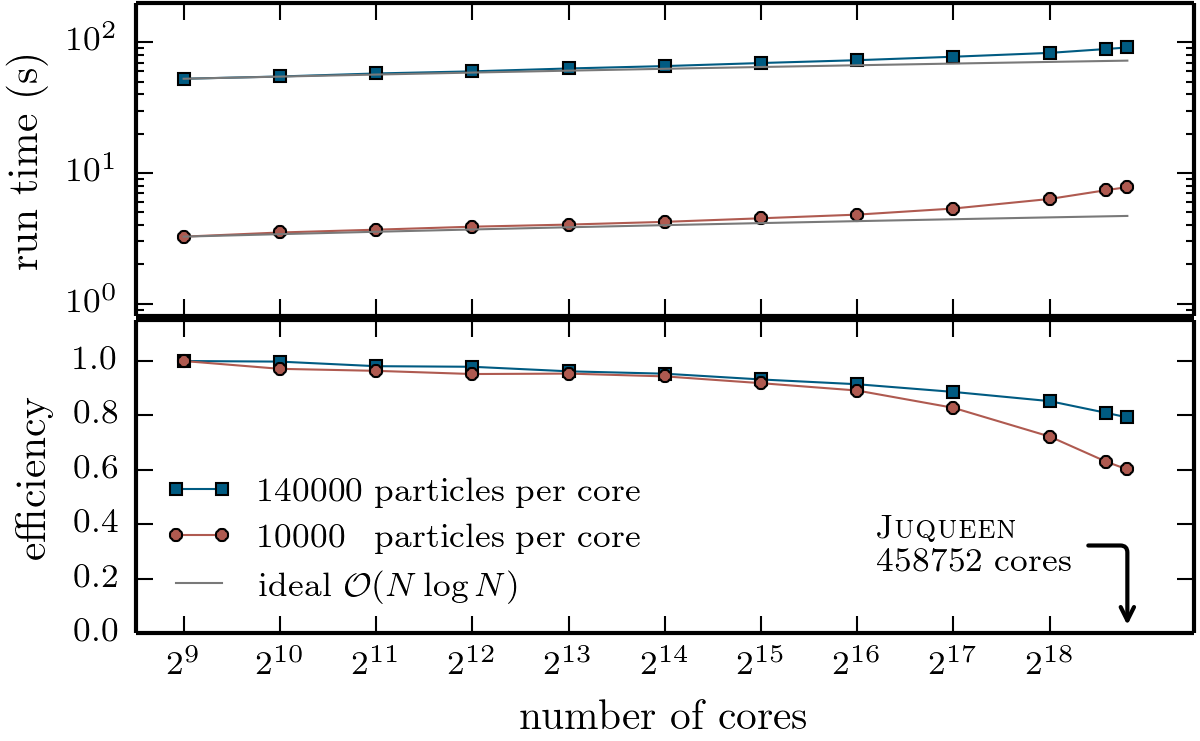
\includegraphics[width=6cm]{Day4/images/weak-good.png}
\end{center}

\column{0.5\textwidth} %second column
\begin{itemize}
	\item {log-log graph}
	\item {runtimes and efficiency on the same graph}
	\item {two different problem sizes}
	\item {complexity order clearly stated}
	\item {Prediction on the largest partition of JUQUEEN}
\end{itemize}
\end{columns}

\textbf{Source: Performance of PEPC \url{http://www.fz-juelich.de/ias/jsc/EN/AboutUs/Organisation/ComputationalScience/Simlabs/slpp/SoftwarePEPC/_node.html}}

\end{frame}



\begin{frame}[containsverbatim]
	\frametitle{Weak scaling : bad example}

\begin{columns}
\column{0.5\textwidth} %first column
\begin{center}
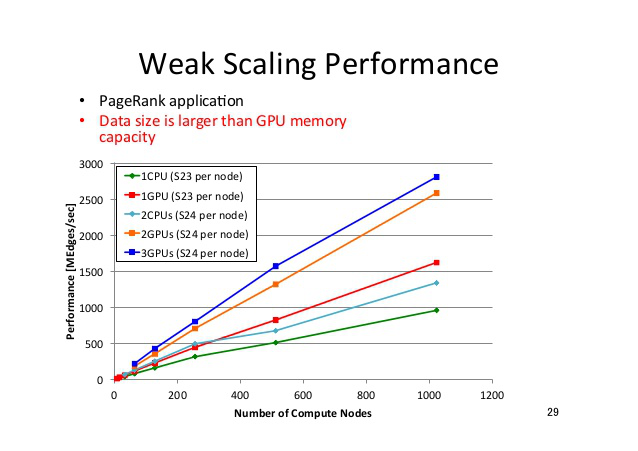
\includegraphics[width=7cm]{Day4/images/weak-bad.png}
\end{center}

\column{0.5\textwidth} %second column
\begin{itemize}
	\item {linear scales}
	\item {no caption}
	\item {``Excel'' look}
	\item {comparison between CPUs and GPUs on the same graph? What is the ``best''? Data does not fit in GPU memory, then?}
\end{itemize}
\end{columns}

\end{frame}



\subsection{Resource budget}


\begin{frame}[containsverbatim]
	\frametitle{Resource budget}

Based on the performance expectations and benchmarks already done, you are able to provide a resource budget for your proposal

\begin{itemize}
	\item { Typical size of problem to solve. Total number of problems to solve }
	\item { Minimum and maximum memory size for the problems }
	\item { Disk space }
	\item { Communications needs (paradigm choice) }
	\item { Architecture }
\end{itemize}
\end{frame}





\begin{frame}[containsverbatim]
	\frametitle{Summary of the Resource Budget}
For the targeted problems
\begin{center}
\begin{tabular}{| l | l |}
	\hline
	Total number of requested cores & 128 - 512 [cores]\\
	\hline
	Minimum total memory & 10 [GB] \\
	\hline
	Maximum total memory & 256 [GB] \\
	\hline
	Temporary disk space for a single run & 100 [GB] \\
	\hline
	Permanent disk space for the entire project & 1 [TB] \\
	\hline
	Communications & Pure MPI \\
	\hline
	License & own code (BSD) \\
	\hline
	Code publicly available ? & Yes \\
	\hline
	Library requirements & LAPACK \\
	\hline
	Architectures where code ran & Intel 64, BG/Q  \\
	\hline
\end{tabular}
\end{center}
\end{frame}



\subsection{Facultative}


\begin{frame}[containsverbatim]
	\frametitle{Facultative add-ons}

\begin{itemize}
	\item { Technical support from the Computing Center (CC)}
	\item { Application-level support from the CC or other institution/groups}
\end{itemize}
\end{frame}





